\documentclass[12pt,letterpaper]{article}

\usepackage[utf8]{inputenc}
\usepackage[spanish]{babel}
\usepackage{times}
\usepackage[left=3cm,top=2.5cm,bottom=2.5cm,right=2.5cm]{geometry}
\usepackage{graphicx}

\title{EV\_ 1\_ 5\_ características de los convertidores de potencia CA-CD, CD-CA, CA-CA y CD-CD}
\author{Perez de Alba Santiago Eduardo}

\begin{document}
\maketitle

\section{Introducción}
Un convertidor de potencia son dispositivos que nos ayudan a transformar la energía eléctrica que se toma de la red, en otro tipo de energía eléctrica necesaria, y que se comporta como un interruptor y que esta construido con semiconductores, ya sean diodos, transistores de potencia, tiristores, GTO, IGBT, BJT, transistores MOSFET, tiristor MCT.
\section{Marco teórico}
\subsection{Convertidores CD-CD(CC-CC):} 


\textbf{Reductor Buck:}
Este destaca por su simplicidad y su elevado rendimiento mayor al (90\%), en este regulador reductor, el voltaje promedio de salida (Va), es menor que el de entrada (Vs).
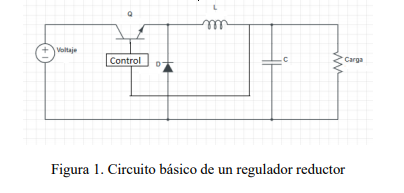
\includegraphics[width= 8cm]{Reductor Buck.png}  
\

\
Este circuito opera de dos maneras:
La primera manera es cuando el transistor(Q) en t=0. La corriente de entrada se eleva y fluye a través del inductor (L), del capacitor (C) y de la resistencia de carga (R).
Segunda manera es cuando se desconecta el transistor (Q) en t=t1. El diodo(D) de marcha libre comienza a conducir debido a la energía que almaceno el inductor y la corriente del mismo continua fluyendo a través del inductor, el Capacitor(C), la resistencia de carga(R) y el Diodo(D). La corriente del inductor para hasta que el transistor vuelve a activarse.

\newpage


Esquemático de cada una de las Operaciones:

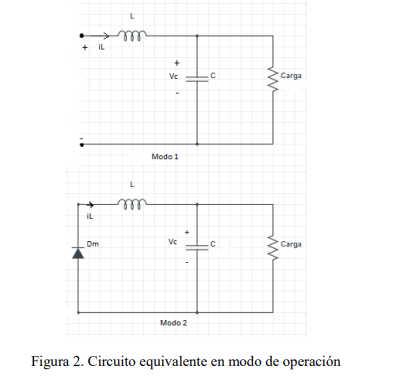
\includegraphics[width=7cm]{Reductor Buck 2 Maneras.png} 

\textbf{Push pull}
\
Este convertidor se deriva del convertidor \textit{Forward}
\

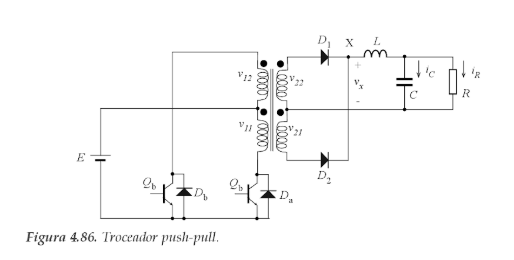
\includegraphics[width=6cm]{PushPull.png} 
\
En la imagen anterior suponen $N_1$ espiras en los devanados primarios y $N_2$ espiras en los secundarios.

Este, utiliza el denominado control decalado, el cual consiste en que a lo largo de un periodo de conmutación, $T_S$, los interruptores controlados permanecen cerrados un tiempo $T_ON$.

En el push-pull viene dada en el primario por dos interruptores controlados ($Q_a y D_b$), con sus respectivos diodos Clamp en antiparalelo ($D_a y D_b$) para permitir la circulación de la corriente de perdidas. En el secundario, dos diodos ($D_1 y D_2$) permiten la circulación de corriente en el circuito de salida únicamente para aportar energía al circuito \textit{LRC} de salida.
\

Cuando el interruptor ($Q_a$) esta cerrado aplica la tension de \textit{E} al primario 1, en el secundario se convierte en tension ($v_22$) de signo positivo, que polariza el diodo ($D_1$) e inversamente el diodo ($D_2$). Esto hace transferencia de energía desde \textit{E} hacia el circuito \textit{LRC} de salida

\

\
\textbf{Convertidor HalfBridge}
\

\
Permite convertir una tension de entrada \textit{E} en otra salida \textit{U}, mayor o menor en función de la relación de espiras del transformador y de la duración de \textit{$T_on$}.
\

\

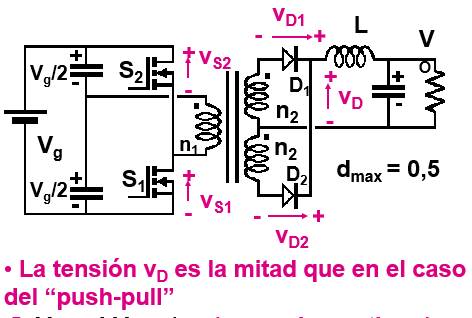
\includegraphics[width=6cm]{Halfbridge.png} 
\

\
Su propósito es distribuir la tension de salida de igual manera, obteniéndose y cuando lo hace se establece sobre el mismo 

\
\

\textbf{Convertidor FullBridge}
\

\
El funcionamiento se da por el cierre y apertura sincronizado de pares de interruptores.
\
$Q_a$ \ y \ $Q_d$ \ en un primer instante se cierran, mientras que $Q_b$ \ y \ $Q_c$ \ permanecen abiertos. esto permite aplicar tension de entrada \textit{E} al primario del transformador, provocando la transferencia de energía al circuito de salida a tras de $D_1$.
\
Cuando los interruptores están abiertos, al abrir por control $Q_a$ \ y \ $Q_b$ \ la tension aplicada al primario es nula, y los diodos $D_1$ \ y  \ $D_2$ \ siguen permitiendo la circulación de la corriente.


\textbf{Reversible en corriente}
\
\


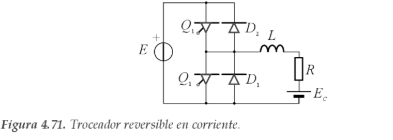
\includegraphics[width=7cm]{Reversible en corriente.png} 

\
El control mas adecuado para la estructura de reversible  en corriente  es denominado control complementario, el cual nos dice que al cerrar el interruptor (transistor Q1) durante el intervalo (0, $ST_S$), manteniendo el interruptor (Q2) abierto, para que en el intervalo ($ST_S$  $T_S$) cerrar el interruptor Q2, y asi mantener el interruptor Q1 abierto.
\
\textbf{Características:}


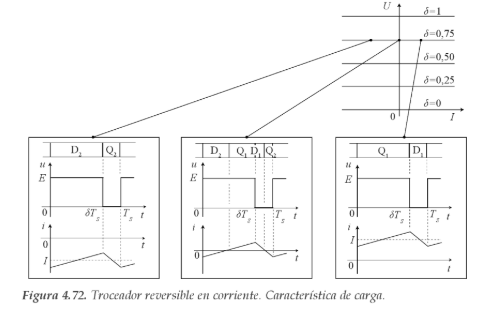
\includegraphics[width=7cm]{Caracteristicas de carga, Reversible en corriente.png} 
\
Lo que se puede observar en la imagen son las ondas de la tension y de la corriente en la carga para tres modos en el cual funciona donde la carga media es positiva, nula o negativa, y también se puede observar el semiconductor que lo conduce en cada instante, el valor medio de la tension en la carga se determina por la siguiente formula:

$$ U= \frac{1}{T_S} \int_{0}^{ST_S} E \ dt \ = SE  $$

\newpage

\textbf{Reversible en Tensión:}
\

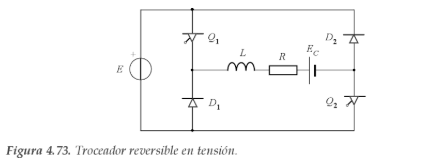
\includegraphics[width=7cm]{Reversible en Tension.png} 
\
El control adecuado para Reversible en Tensión es denominado control simultaneo, que consiste en cerrar ambos interruptores (Transistores Q1 y Q2) simultáneamente durante el intervalo (0,$ST_S$) y mantenerlos abiertos durante el intervalo ($ST_S  \  T_S $)

En la siguiente imagen se muestran las formas de onda de la tension y la corriente, en donde la tension media en la carga es positiva, nula o negativa.
\

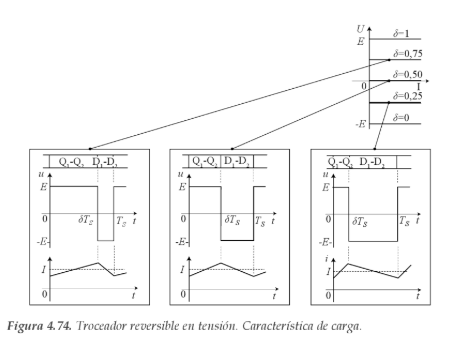
\includegraphics[width=7cm]{Caracteristicas de carga.png} 


\
La formula que representa los valores medios de la tension en la carga es la siguiente:
\

\textbf{Reversible en tension y Corriente (Puente completo)}
\

\
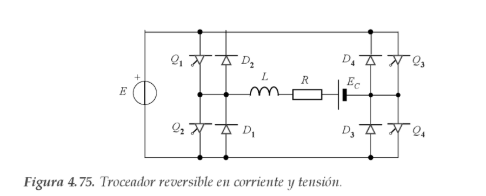
\includegraphics[width=8cm]{Full bridge.png} 

\
Para esta estructura, aplicada a la conversión CC-CC, el control más adecuado es el Control Complementario, que consiste en cerrar los interruptores (Transistores Q1, Q4) durante el intervalo (0, $ST_S$) manteniendo abiertos los interruptores (Transistores Q2, Q3) para luego proceder a cerrar los interruptores (Transistores Q2, Q3) durante el intervalo ($ST_S$ \ $T_S$) y de esta manera mantener los interruptores (Transistores Q1, Q4).
\newpage
Dando como resultado las siguientes formas de onda:
\

\
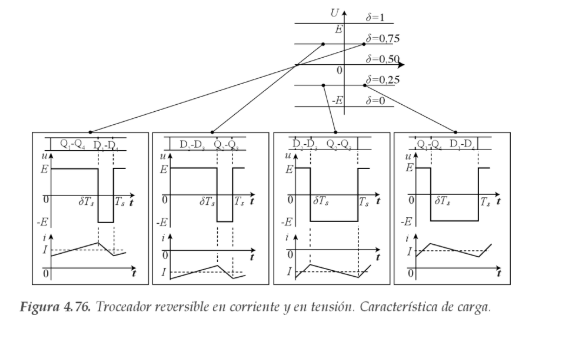
\includegraphics[width=8cm]{Caracteristicas de carga Full Bridge.png} 
\

Donde se puede observar la forma de onda de la tension y de la corriente en la carga para el caso de una máquina eléctrica que, en los dos sentidos de giro puede trabajar como motor o como generador.
En el primer cuadrante, la potencia absorbida es positiva. La maquina estara en fase de tracción. Modificando el signo de la corriente.
En el segundo cuadrante, La potencia absorbida es negativa. donde la carga trabaja como generador.
En el tercer cuadrante, se modifica la relación de conducción "S", cambia el signo de la tensión situándose el punto de funcionamiento.
En el cuarto cuadrante, el cambio del signo de la corriente situará el punto de funcionamiento, en el que la potencia es negativa.


\
\textbf{Convertidor Forward (2 interruptores)}
\

\
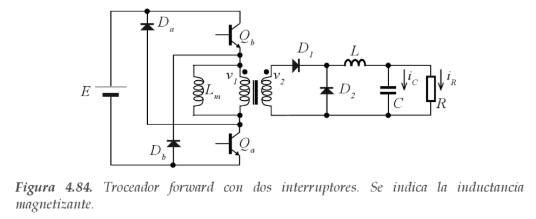
\includegraphics[width=6cm]{Forward.png} 

\

\
Esta estructura funciona de manera que ambos transistores se mueven simultáneamente, de forma que cuando estos están cerrados, los diodos $D_a$ y $D_b$, denominados trampa \textit{Clamp} están abiertos, la tension en el primario del transformador vale E, la corriente magnetizante crece, y se transfiere energía a la carga ya que $D_1$ permanece cerrado. Mientras que los transistores están abiertos $D_1$ también lo esta, conduciendo $D_a$ y $D_b$, aplicándose en el primario del transformador una tensión de -E que hace que la corriente magnetizante decrezca.
\

\newpage
\textbf{Elevador boost}

\
Destaca por su simplicidad y su elevado rendimiento, sin embargo, es difícil de estabilizar en lazo cerrado y presenta una respuesta transistoria de baja calidad. Su característica elevadora de tension se ve afectada por la resistencia de la inductancia. el rizado de la tension de salida es peor que en el reductor, y las corrientes eficaces que soportan los semiconductores

\

\

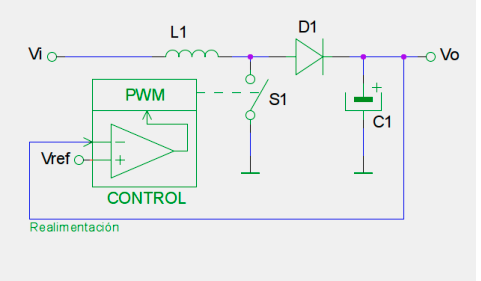
\includegraphics[width=6cm]{Elevador Boost.png} 
\

\

\textbf{Reductor-Elevador}

\
El funcionamiento de este convertidor es de dos maneras:
La primer manera es cuando esta encendido, la fuente de entrada de voltaje esta directamente conectada al inductor (L). Por lo que se almacena energía en L. Con esto, el condensador proporciona corriente a la carga de salida.
La segunda manera es cuando esta apagado o en estado off, el inductor esta conectado a la carga de salida y el condensador, por lo que la energía es transferida del inductor (L) al capacitor (C) y a la resistencia (R).
\

\
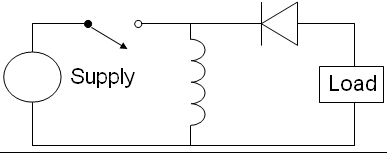
\includegraphics[width=6cm]{Reductor-Elevador.png} 





\

\
\textbf{Convertidor Flyback (2 interruptores)}

\

\
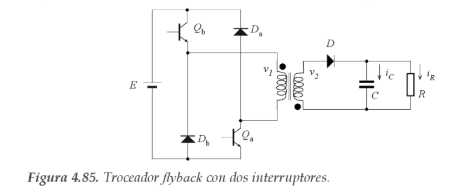
\includegraphics[width=6cm]{Flyback.png} 
\
Es similar al convertidor forward, en este se utiliza el transistor como se muestra en la imagen.
Teniendo en cuenta que se mantiene la relación de conversión del convertidor que, en modo conducción continua, esta dada por la siguiente formula:
$$U= \frac{S}{1-S} \frac{N_2}{N_1}E$$

\

\



\textbf{Convertidor Cuk}
\

\
El condensador C transfiere energía y se conecta alternativamente a la entrada y a la salida del convertidor a través de la conmutación del transistor y el diodo.
las dos bobinas $L_1$ y $L_2$ son usadas para convertir la fuente de entrada de voltaje y la fuente de voltaje de salida en fuentes de corriente.
\

\







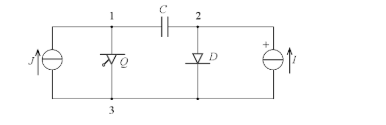
\includegraphics[width=6cm]{Convertidor Cuk.png} 

\

\
\subsection{Convertidores CC-CA:}

\textbf{Alimentado en tension:}
\
La fuente primaria suele ser un sistema de comportamiento cercano al de la batería, es decir, de bajo rizado de tension, capaz de imponer a la carga mediante la actuación de los interruptores del ondulador, una o varias tensiones de valor nulo. la carga es un receptor inductivo

\

\

\textbf{Alimentado en corriente:}

El comportamiento de la fuente de corriente se utiliza para implementar a partir de un sistema de comportamiento parecido al de una bateria, a la cual se le conecta en serie una bobina para disminuir el rizado de corriente de entrada. En este caso, la carga es un receptor de tension.


\

\

\textbf{Conversor Monofasico:}
\
En este circuito o esquema existen 4 interruptores de potencia, que trabajan en base a patrones de conmutación establecidos. Donde siempre habra dos interruptores trabajando.
\

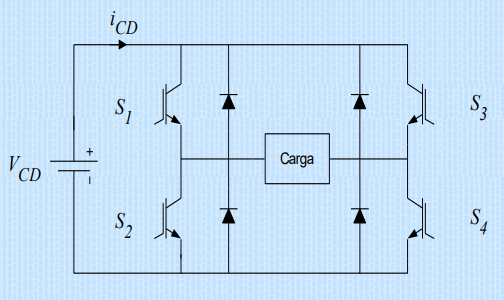
\includegraphics[width=6cm]{Monofasico.png}

\ 

\subparagraph{ 1.-Semi-Puente (halfbridge::}
\

\
Este convertidor pretende aplicar una resistencia a una tension de valor medio variable. y este sistema es capaz de aplicar a la salida una tension \textit{u(t)} \ positiva \textit{($S_1$ \ cerrado} o nula \textit{($S_1$ \ abierto}, con lo que dicha tension es unipolar.
Tensión de salida bipolar: Se tiene que conectar en anti-paralelo con la carga, y según $S_2$ este cerrado o abierto, es capaz de aplicar, por si solo en la carga, una tension de salida negativa o nula.
En este circuito $S_1$ \ y \ $S_2$ \ no pueden estar simultáneamente cerrados, sino se daría un cortocircuito en las fuentes de tension
\
\

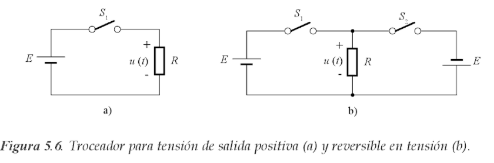
\includegraphics[width=6cm]{Semi-puente.png} 
\

\

\textbf{2.-Puente completo:}
\

\
Esta formado por dos ramas onduladoras de tension $S_1-S_2$ \ y \ $S_3-S_4$, con $f_s$ = $f_1$ \ la frecuencia de conmutación, y la finalidad de imponer en la carga una tension \textit{u(t)} de valor medio nulo.
\
Existen dos formas básicas de control de esta estructura según que el control imponga una salida bipolar en la carga o imponga una tension de salida en zonas muertas de tension nula en la carga.
\

Onda cuasi-cuadrada: Esta permite variar el valor eficaz de la tension de salida y dicha tension contiene armónicos de diferente amplitud.
\

Onda cuadrada:  Este permite dar como resultado una corriente en la carga de valor máximo, eficaz y contenido de armónicos análogos.
\

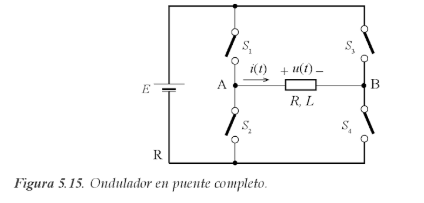
\includegraphics[width=6cm]{Puente completo.png} 

\


\

\textbf{3.-Push-Pull:}
\
Es ondulador de cuadrada ya que utiliza un control complementario de los interruptores, soportando una tension que es el doble de la tension de la batería.


\

\
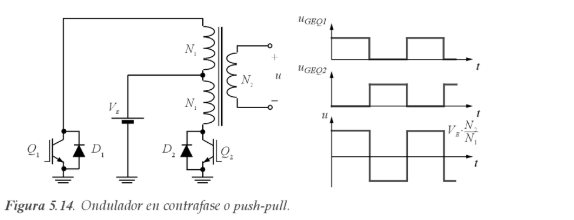
\includegraphics[width=6cm]{Push Pull CC-CA.png} 
\

\

\textbf{Convertidor trifásico:}
\
Los inversores trifásicos se emplean en aplicaciones de baja, media y alta potencia, con tensiones de salida de baja y media tension.

En aplicaciones de baja tension, la salida de potencia es tomada directamente del puente inversor.
En aplicaciones de media tension, Se necesita emplear un transformador elevador cuya función es escalar la tension a los niveles necesarios.

En este esquema no existe un neutro de forma natural. En cargas donde es necesaria su conexión, se emplea un transformador delta-estrella en la salida.
\
Este esta compuesto por 6 transistores, cada uno con un diodo en conexión inversa, empleados para conducir la corriente reactiva de retorno a la fuente de tension E. Se dividen según su forma de operar: en conducción a 180 grados de cada elemento, con lo cual hay 3 elementos en conducción al mismo tiempo y conducción 120 grados, con dos elementos por vez.

\

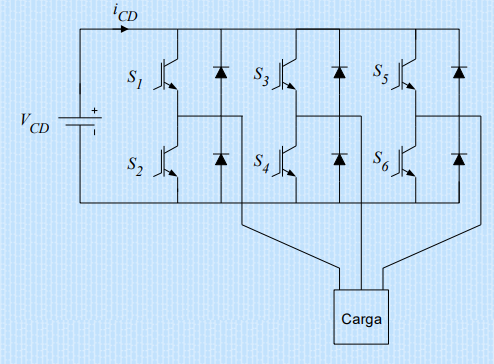
\includegraphics[width=7cm]{Trifasico.png} 
\

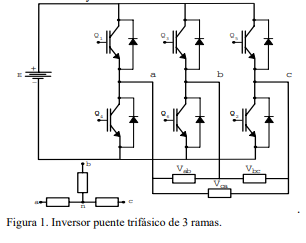
\includegraphics[width=7cm]{Delta-Estrella.png} 
\

\
\textbf{Forma de onda de salida:}
\
\subparagraph{1.-Cuadrada:}
\
Esta es una técnica de modulación y el esquema al que se le asocia es al del inversor de puente completo, ya que es el que genera una tension de salida en forma de onda cuadrada.
En este caso los interruptores conectan la carga "a" + $V_cc$ \ cuando $S_1$ \ y \ $S_2$ \ están cerrados (estando \ $S_3$ \ y \ $S_4$ \ abiertos) y "a" - $V_cc$ \ cuando $S_3$ \ y \ $S_4$ \ están cerrados  (Estando \ $S_1$ \ y \ $S_2$ \ abiertos). La conmutación periódica de la tension de carga entre + $V_cc$ \ y \ - $V_cc$ genera en la carga una tension con forma de onda cuadrada.
\
La forma de onda de la corriente en la carga depende de los componentes de la carga.

\
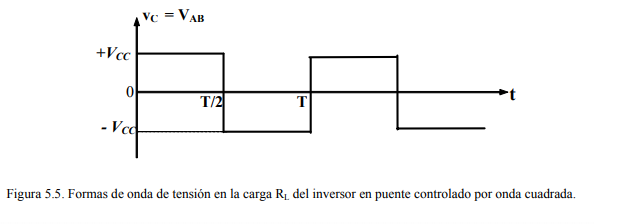
\includegraphics[width=7cm]{Onda cuadrada.png} 

\

\subparagraph{2.- Cuasi-Cuadrada:}
\
Esta onda mantiene un nivel de tension nulo sobre la carga durante parte del periodo. De esta manera se mejora el contenido de los armónicos de la tension de salida.
\
Esta se obtiene: que cuando se desea tension positiva en la carga se mantienen $S_1$ \ y \ $S_2$ \ conduciendo ($S_3$ \ y \ $S_4$ \ abiertos). La tension negativa se obtiene de forma complementaria ($S_3$ \ y \ $S_4$ \ cerrados y \ $S_1$ \ y \ $S_2$ \ abiertos).
Para obtener la tension nula a la salida es manteniendo todos los interruptores abiertos durante el intervalo de tiempo deseado.
\

\
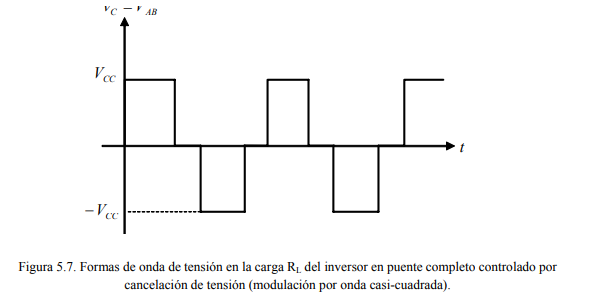
\includegraphics[width=7cm]{Onda Cuasi-Cuadrada.png} 
\

\
\subparagraph{3.- Moduladas:}
\
Este se utiliza para mejorar el contenido de armónicos en la salida de un inversor.
Su idea básica esta en comparar una tension de referencia senoidal de baja  con una señal triangular simétrica de alta frecuencia cuya frecuencia determine la frecuencia de la conmutación.
La frecuencia de la onda triangular debe ser, como mínimo 20 veces superior a la máxima frecuencia de la onda de referencia, para que se obtenga una reproducción aceptable de la forma de onda sobre una carga.
Apartir de la señal modulada se generan los pulsos de apertura y cierre de los interruptores, es decir si la señal modulada tiene un valor alto, los interruptores $S_1$ \ y \ $S_2$ \ se cierran. En caso contrario los interruptores $S_3$ \ y \ $S_4$ \ se cierran.
\

\

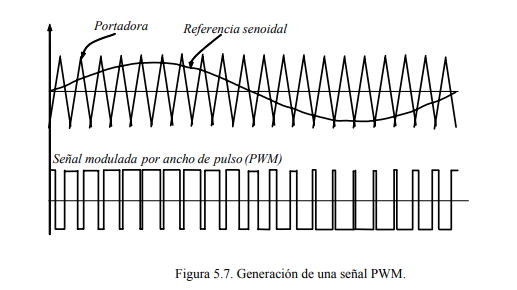
\includegraphics[width=6cm]{Modulada.png}
\

\
\subparagraph{4.- Resonantes Multinivel:}
\

Los convertidores  multinivel son una opción de conversión de energía en el rango de media-alta potencia.
Son sintetizadores de tension. La tension alterna de salida, de valor elevado, se sintetiza a partir de diferentes niveles de tension continua de entrada, de valor mas pequeño, accionando apropiadamente los interruptores del convertidor.
\

\
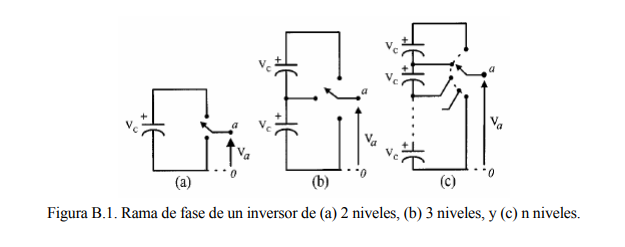
\includegraphics[width=7cm]{Multinivel.png}   
\

\
\subsection{Convertidores CA-CA:}
\

\
\subparagraph{1.- Variadores de CA:}
\

Es utilizada para mejorar la eficiencia energética, donde la energía de la red pasa por el variador y regula la energía, reduce la potencia de salida.
\
Estos funcionan mediante la conversión de alimentación CA de frecuencia fija en frecuencia variable, variable de tension de alimentación de CA.
\

Toma alimentación eléctrica de la red, cual tiene voltaje y frecuencia fija, la transforma en voltaje continuo y luego lo transforma en voltaje alterno trifasico de magnitud y frecuencia variable por medio de un inversor
\


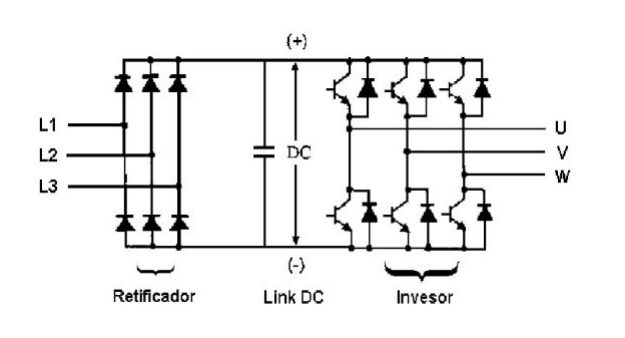
\includegraphics[width=7cm]{Variadores CA.png} 
\

\subparagraph{2.- Ciclo controladores:}

\

Los ciclocontroladores pueden mejorar la calidad de salida de corriente y el factor de potencia de entrada de amplitud de pulso modulación de control de corriente alterna, y así mejorar los armónicos 




\

\subparagraph{3.-Convertidores Matriciales:}
\
El convertidor Matricial forma parte del sistema de potencia de una sola etapa, con linea de alimentación de CA de tipo trifasica y una carga trifasica.

\

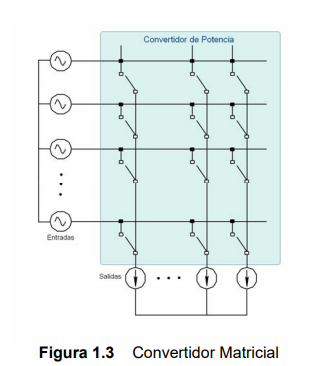
\includegraphics[width=6cm]{Convertidor matricial.png}
\

\
Gracias al arreglo de interruptores, la potencia en el convertidor puede ser reversible. Esto debido a que no existen elementos que almacenen energía, la potencia instantánea de la entrada debe ser igual a la potencia en la salida.
\

\

\subsection{Convertidores CA-CD:}
\

Estos proporcionan una señal de salida rectificada de valor Vm que es igual al Vp del voltaje de entrada. Y utilizan el transistor como un control.
\

\
\subparagraph{1.-No controlados:}
\

Nos dice que no se puede controlar la magnitud de la tension continua, siempre se mantiene fija. 
\

El objetivo de este convertidor es transformar la tension alterna en continua, es decir, si la tension alterna de entrada tiene una frecuencia y valor eficaz constante, y se pretende conseguir una tension continua de salida en todo momento.
En este se tiene un inductor conectado a otros dos, que van directamente al diodo en la misma dirección 

\

\



\

\subparagraph{2.- Controlados:}
\

En los circuitos rectificadores se puede sustituir el total o parcial a los diodos por tiristores, obteniendo un sistema de rectificación controlado.
\

La puerta es la encargada de controlar el paso de corriente entre el anodo y el catodo, permitiendo circular la corriente en un solo sentido.

\



\end{document}